% *********** Frequency Analysis **********
% - Blabla
% *****************************************

\subsection{Frequency Analysis}
Frequency analysis is a powerful tool for examination of the behaviour of dynamic systems. Hopsan has built-in support for producing bode diagrams as well as frequency spectrums. Both of these are calculated by converting variables from time domain to frequency domain by using fast fourier transforms (FFT).

\subsubsection{Frequency Spectrum}
A frequency spectrum is a frequency domain diagram that shows the frequency contents of a signal. Consider a signal $x(t)$. This is transformed to frequency domain by FFT:\\

$X(i\omega)=FFT(x(t))$\\

The amplitude for each frequency can thus be calculated as the absolute value of the complex signal. Finally, we want the amplitude squared (known as a \textit{power spectrum}).\\

$P(i\omega)=abs(X(i\omega))^2$\\

Frequency spectrums in Hopsan are created from inside the plot window. First plot the desired signal in time domain, and then click the "FFT" button in the curve settings panel to the right.


\begin{SCfigure}[12][h]
  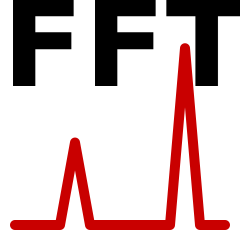
\includegraphics[width=5mm]
    {../../HopsanGUI/graphics/uiicons/Hopsan-FrequencyAnalysis.png}% picture filename
  \caption*{Create frequency spectrum from plot curve}
\end{SCfigure} 
\subsubsection{Bode Diagrams}
A bode diagram contains information about gains and phase shift for different frequencies. For doing this we first need to extract a transfer function from the model. Suppose we have a linear system with input and output variables $x(t)$ and $y(t$. In the frequency domain, the transfer function will be the relationship between these variables:\\

$Y(i\omega)=G(i\omega)X(i\omega)$ \\

where $G(i\omega)$ is the transfer function, $X(i\omega)$ the fourier transformed input signal  $Y(i\omega)$ the fourier transformed output signal, $\omega$ the frequency and $i$ the square root of $-1$. The transfer function can thus be obtained from\\

$G(i\omega)=\frac{FFT(y(t)}{FFT(x(t)}$\\

This will give a vector of complex numbers from where the magnitude is calculated from the absolute value and the phase shift from the argument. The frequency range is limited as follows, due to the Nyquist frequency: \\

$\frac{1}{\Delta T}<f_{bode}<\frac{n_{samples}}{\Delta T}$\\

Here $\Delta T$ is the simulated time and $n_{samples}$ the number of log samples used.

%Todo: Conditions
%Todo: How to do it

\begin{SCfigure}[7][h]
  %\centering
  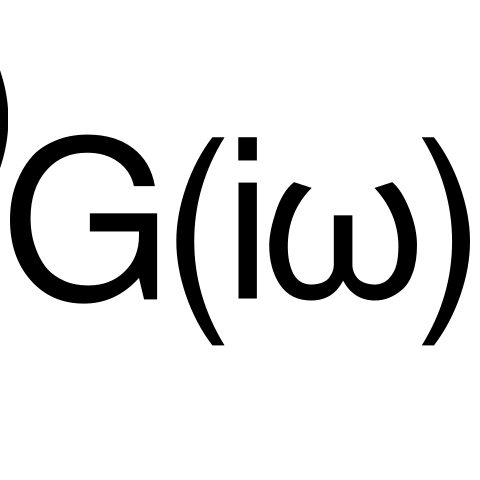
\includegraphics[width=5mm]
    {../../HopsanGUI/graphics/uiicons/Hopsan-TransferFunctionAnalysis.png}% picture filename
  \caption*{Create a bode diagram}
\end{SCfigure}



% *********** Frequency Analysis **********
